

\begin{frame}{Bonnes pratiques dans le numérique}{Conseils 102-105/115}
\begin{block}{Utiliser la version la plus récente du langage}
Les langages côté serveurs (PHP, Ruby, Java) sont régulièrement améliorés par les différentes communautés (performances, de gestion mémoire, de stabilité et comble des failles de sécurité).
\end{block}

\begin{block}{Ne charger des données/du code que lorsqu'elles sont/il est nécessaire}
Les préchargements gaspillent des ressources.
\end{block}


\begin{block}{Éliminer les fonctionnalités non utilisées}

Piloter/supprimer certains usages de fonctionnalités.

\end{block}


\begin{block}{PWA > application mobile native similaire au site web}
 Définir les supports nécessaires en fonction des utilisateurs. Un site internet responsive peut-être tout à fait suffisant et satisfaisant.
\end{block}

\end{frame}

\begin{frame}{Bonnes pratiques dans le numérique}{Conseils 106-109/115}
\begin{block}{Éviter les temps de blocages par des traitements javascript trop longs}
 Découper vos JavaScript en petites tâches exécutées au moment requis et non pas avant.
\end{block}

\begin{block}{Mettre en place une architecture élastique}
 Modifier dynamiquement et automatiquement la taille de l'infrastructure en fonction de la charge. 
\end{block}


\begin{block}{Éliminer les fonctionnalités non utilisées}

Piloter/supprimer certains usages de fonctionnalités.

\end{block}


\begin{block}{Limiter le nombre d'appels aux API HTTP}
Fixer des quotas afin d'inciter les utilisateurs à définir une stratégie de mise en cache des réponses et éviter des appels systématiques. 
\end{block}

\end{frame}



\begin{frame}{Bonnes pratiques dans le numérique}{Conseils 110-114/115}
\begin{block}{Limiter le recours aux carrousels}
Limiter au maximum l'utilisation des carrousels en privilégiant du contenu statique mis à jour régulièrement. 
\end{block}

\begin{block}{Avoir une stratégie de fin de vie des contenus}
Supprimer les contenus non utilisés. 
\end{block}


\begin{block}{Mettre en place un "Circuit breaker"}
Un "circuit breaker" casse le traitement d'une requête à travers plusieurs services dans le cas où un des services ne répond pas.

\end{block}


\begin{block}{Favoriser le "Request collapsing"}
Limiter le nombre d’appels distants en regroupant plusieurs requêtes pour n’en faire qu’une seule.
\end{block}

\end{frame}


\begin{frame}{Pause débunkage }{L'agriculture}
%https://www.contrepoints.org/2022/05/05/380845-comment-lagro-ecologie-va-affamer-des-millions-de-personnes

\begin{figure}
    \centering
    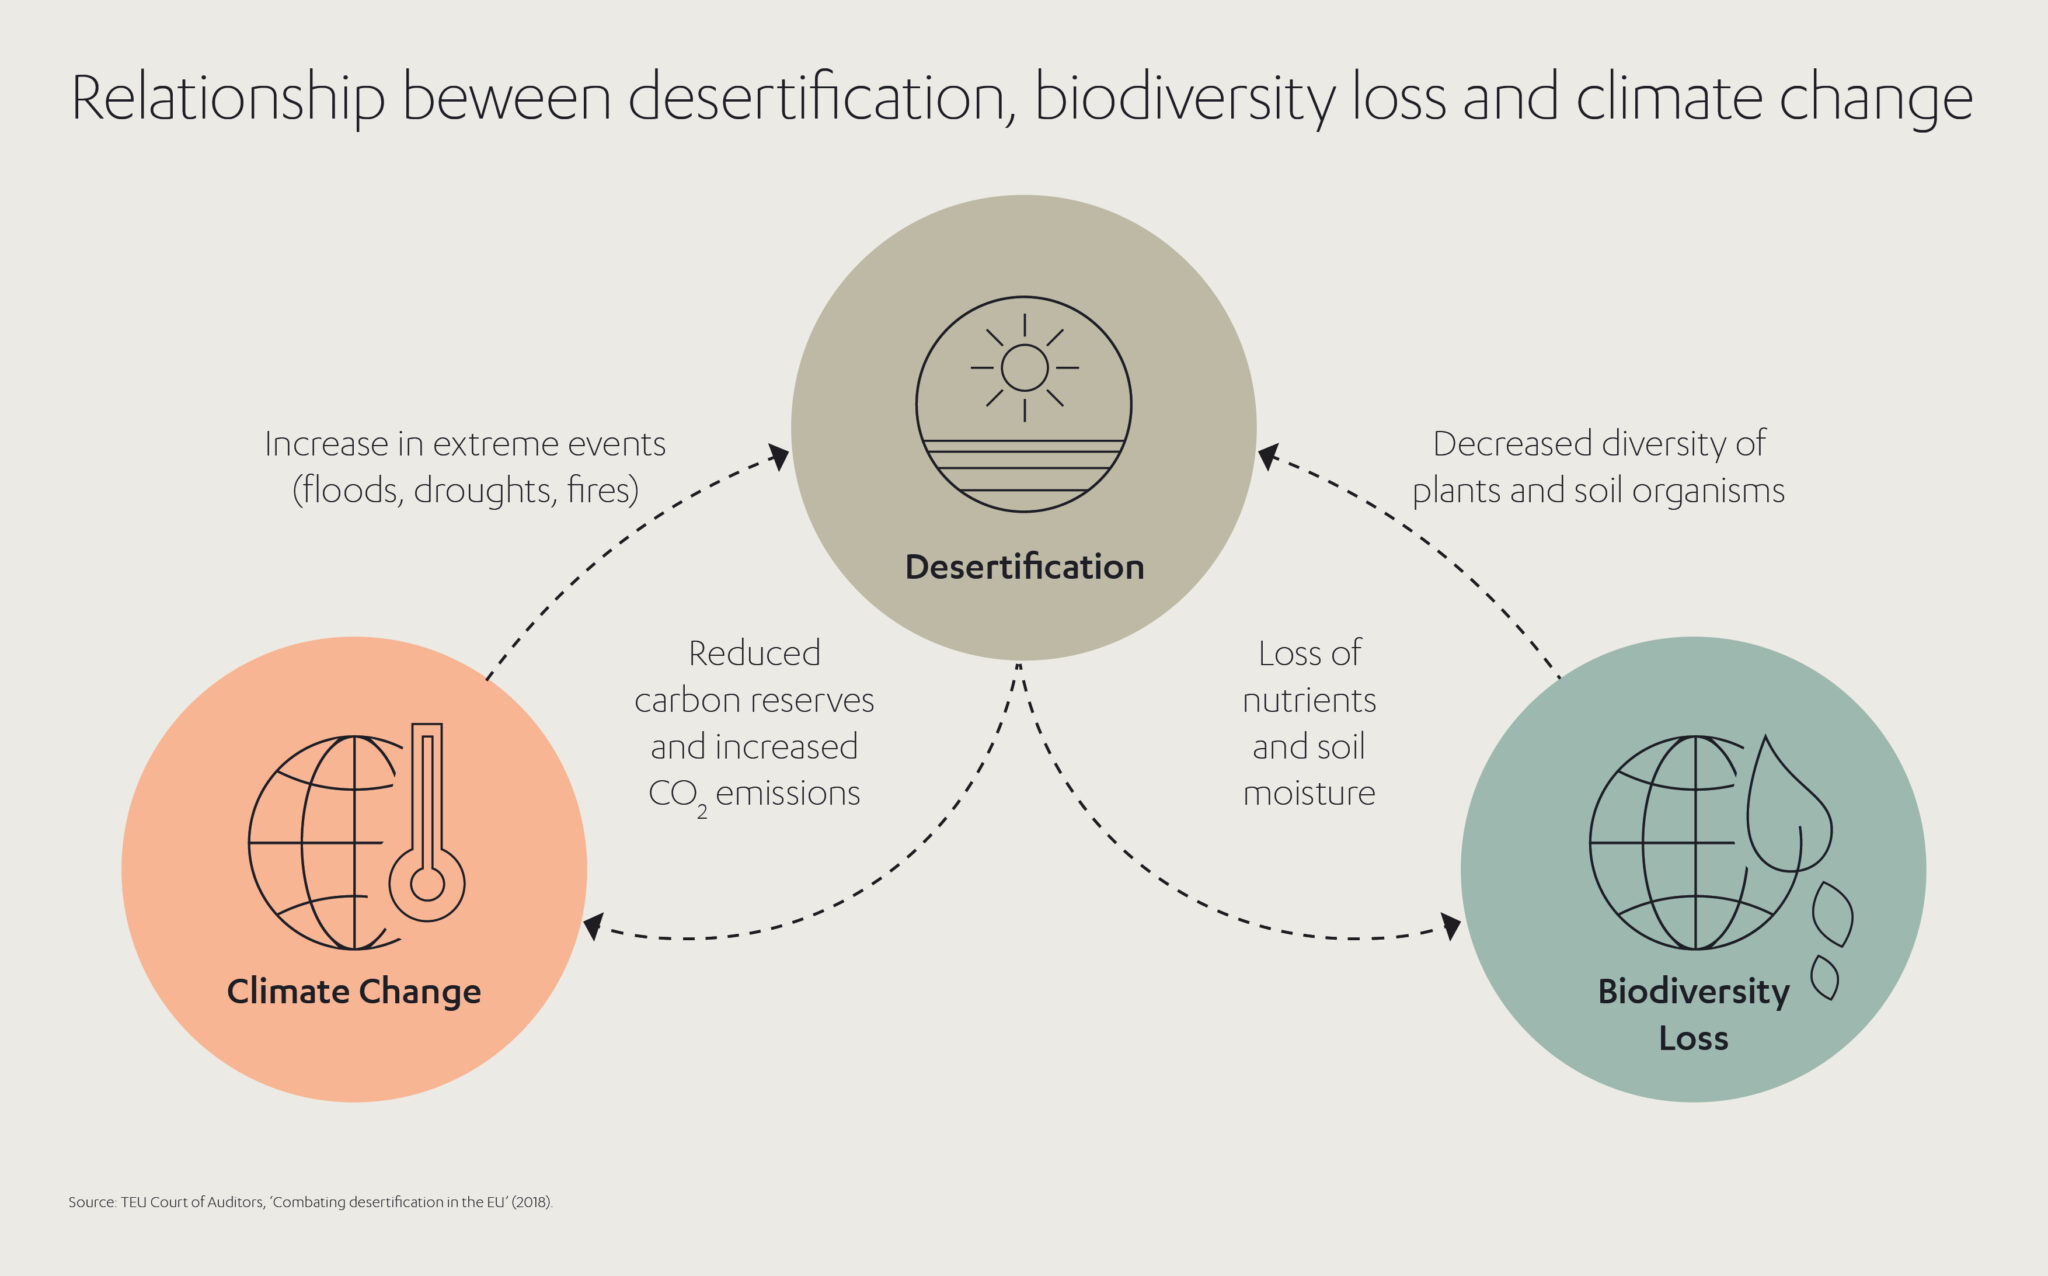
\includegraphics[scale=0.5]{chapitre2/wdd9/fig/agri.jpg}
\end{figure}
\end{frame}


\begin{frame}{Bonnes pratiques dans le numérique}{Conseil 115/115}
\begin{block}{Ne pas afficher les documents à l'intérieur des pages}
Pour être affiché, un fichier de traitement de texte devra, par exemple, appeler un logiciel adapté. Or si ce logiciel n'est pas installé sur le poste de l'utilisateur, le fichier ne pourra pas être lu sans un développement spécifique coûteux. Il est donc préférable d'insérer un lien de téléchargement du document à l'intérieur de votre page afin que seuls les utilisateurs concernés le téléchargent.
\end{block}

\end{frame}

\begin{frame}{Bonnes pratiques dans le numérique}{Comment faire un site éco-responsable ? Côté serveur}
%-------------------------------------------------------
\begin{block}{Quelques PUE, proximité}

\begin{minipage}[b]{0.6\linewidth}

\begin{itemize}
\item Infomaniak
\item Planethoster
\item Ikoula
\item Varnish
\item Web Engine
\item Hostpapa 
\item Ionos (1\&1)
    %\item Un fond sombre demande moins de ressources qu’un fond blanc. 
    %\item Privilégier les animations 2D aux 3D. Elles sont moins gourmandes en ressources.
    %\item Les vidéos utilisent beaucoup de bandes passantes sur les serveurs. Il vaut mieux utiliser des visuels légers.
    %\item Pour avoir une empreinte carbone faible, un site web éco-responsable doit être composé de texte et d’illustrations.
    %\item Dans le choix de format pour les photos, il est préférable d’opter pour le WebP, WebM ou SVG. JPG, Png et Mp4 sont à utiliser en dernier recours.
\end{itemize}
Regarder si compression Gzip accessible

\end{minipage}\hfill
\begin{minipage}[b]{0.35\linewidth}  
\begin{figure}
    \centering
    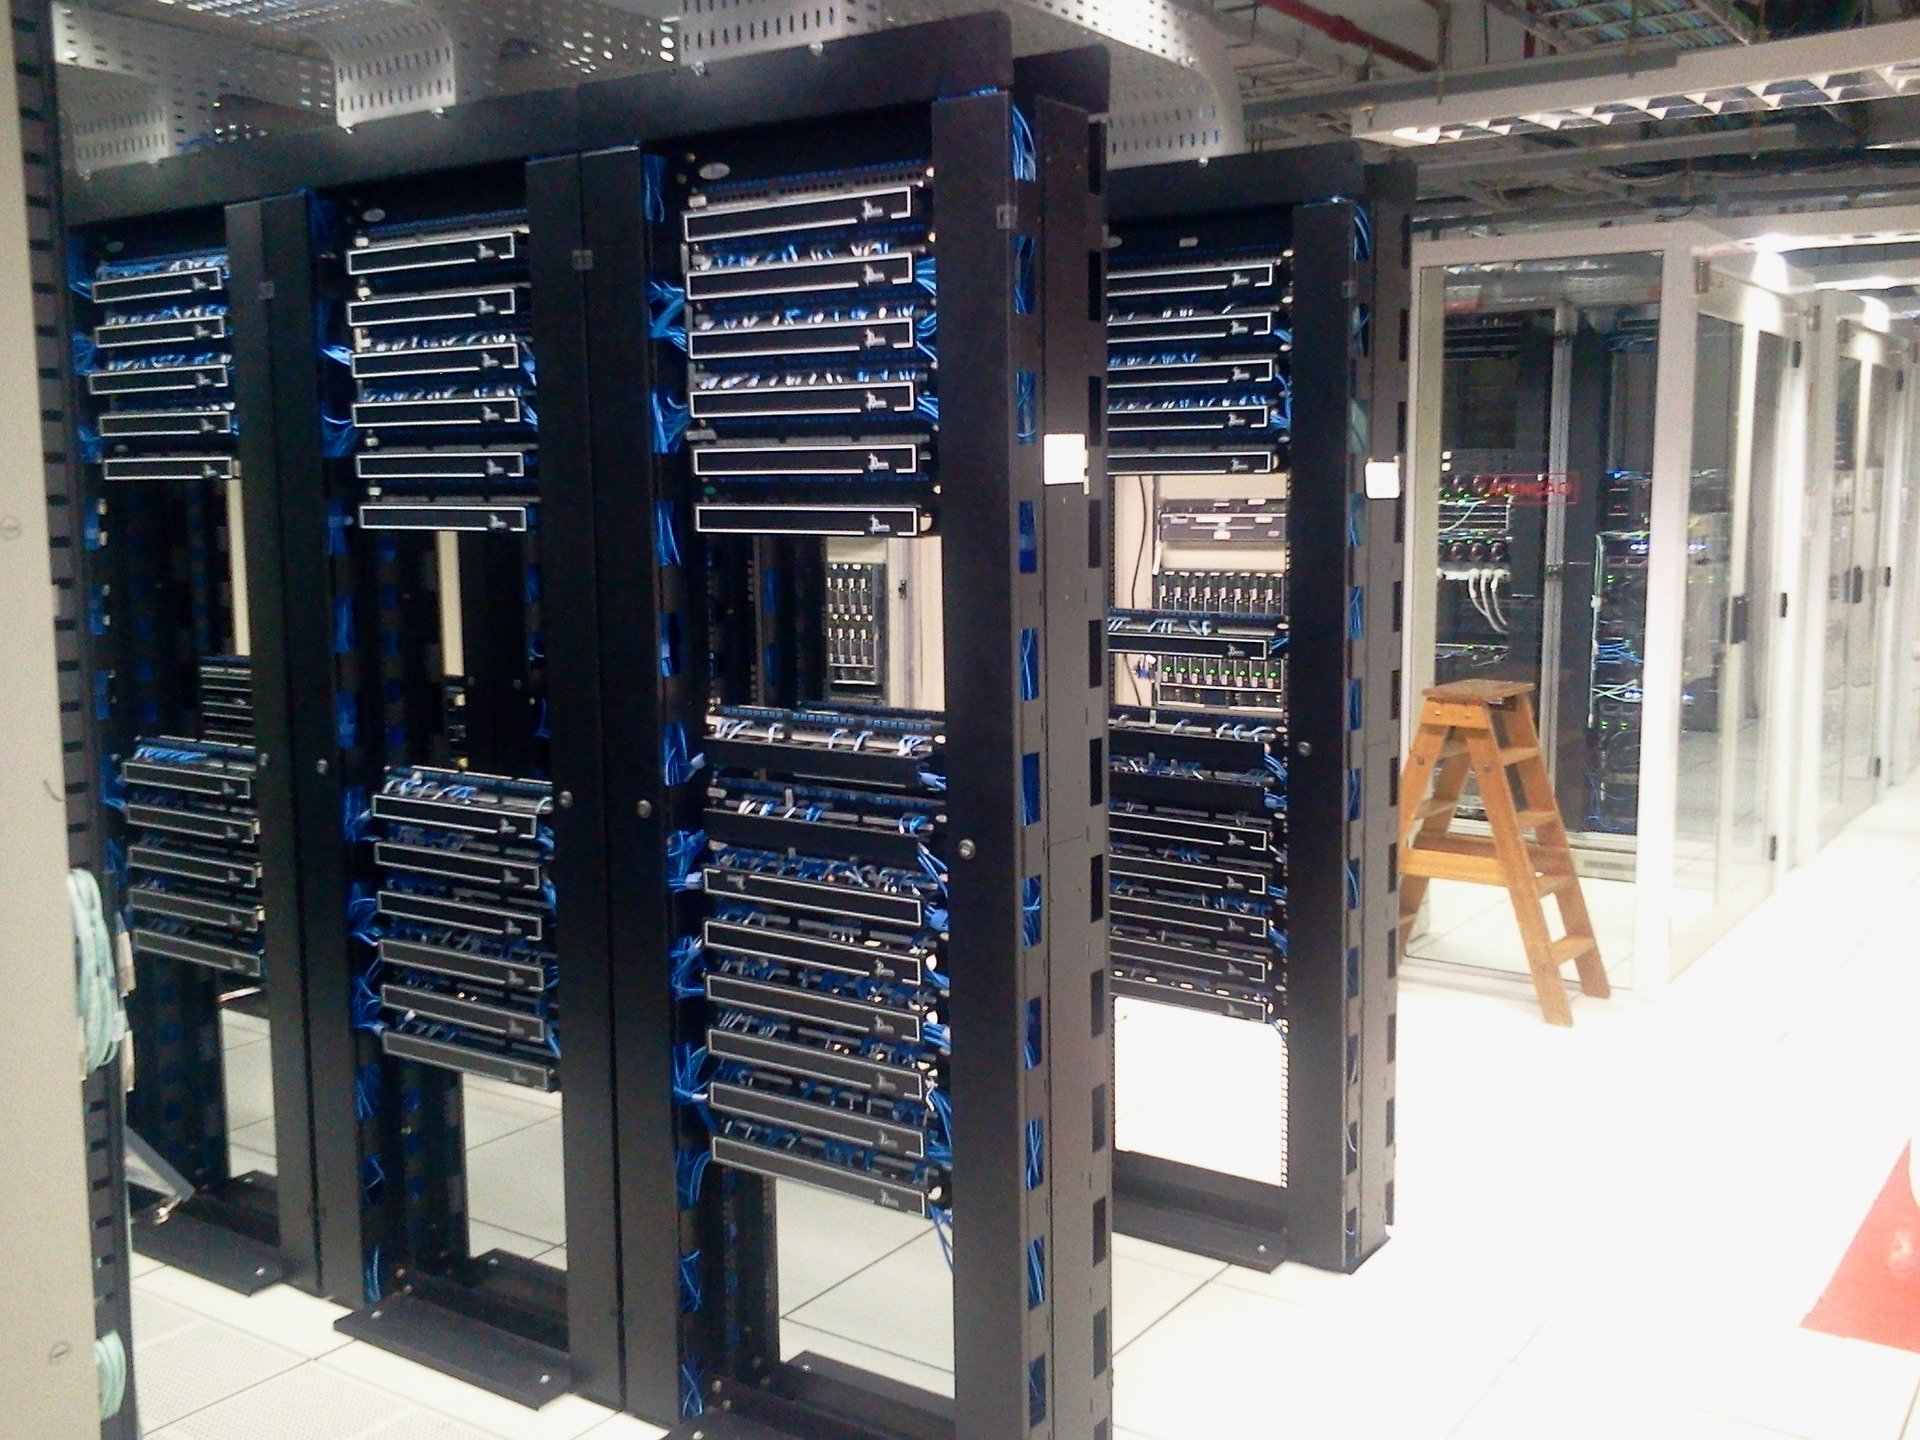
\includegraphics[scale=0.05]{Feathergraphics/datacenter.jpg}
\end{figure}
\end{minipage}\hfill
\end{block}
\begin{block}{Et comment connaitre con empreinte carbone ?}

\url{https://www.websitecarbon.com/}
\end{block}

\end{frame}